%%%%%%%%%%%%%%%%%%%%%%%%%%%%%%%%%%%%%%%%%%%%%%%%
%% Compile the master file!
%% 		Slides: Antonio Machicao y Priemer
%% 		Course: Wissenschaftliches Arbeiten
%%%%%%%%%%%%%%%%%%%%%%%%%%%%%%%%%%%%%%%%%%%%%%%%


%%%%%%%%%%%%%%%%%%%%%%%%%%%%%%%%%%%%%%%%%%%%%%%%%%%%
%%%             Metadata                         
%%%%%%%%%%%%%%%%%%%%%%%%%%%%%%%%%%%%%%%%%%%%%%%%%%%%  

\title{
	\LaTeX\ for Linguists
}

\subtitle{\LaTeX\ 1: Basics}

\author[aMyP]{
	{\small Sebastian Nordhoff \& Antonio Machicao y Priemer}
	\\
	{\footnotesize \url{www.linguistik.hu-berlin.de/staff/amyp}}
	%	\\
	%	{\footnotesize \href{mailto:mapriema@hu-berlin.de}{mapriema@hu-berlin.de}}
}

\institute{LOT 2019, Amsterdam}

%\date{ }

%\publishers{\textbf{6. linguistischer Methodenworkshop \\ Humboldt-Universität zu Berlin}}

%\hyphenation{nobreak}


%%%%%%%%%%%%%%%%%%%%%%%%%%%%%%%%%%%%%%%%%%%%%%%%%%%%
%%%             Preamble's End                   
%%%%%%%%%%%%%%%%%%%%%%%%%%%%%%%%%%%%%%%%%%%%%%%%%%%%      


%%%%%%%%%%%%%%%%%%%%%%%%%%%%%%%%%%%
%%%%%%%%%%%%%%%%%%%%%%%%%%%%%%%%%%%    
%% Title slide 
\begin{frame}
  \HUtitle
\end{frame}


%% Contents slide
\frame{
\begin{multicols}{2}
	\frametitle{Inhaltsverzeichnis}
%	\tableofcontents[hideallsubsections]
	\tableofcontents
	%[pausesections]
\end{multicols}
	}


%%%%%%%%%%%%%%%%%%%%%%%%%%%%%%%%%%%%
%%%%%%%%%%%%%%%%%%%%%%%%%%%%%%%%%%%%
%% Extra literature

\nocite{Freitag&MyP15a}
\nocite{Knuth1986}
\nocite{Kopka94a}
\nocite{MyP17c}
\nocite{MyP&Kerkhof16a}
	
%%%%%%%%%%%%%%%%%%%%%%%%%%%%%%%%%%%%
%%%%%%%%%%%%%%%%%%%%%%%%%%%%%%%%%%%%


%%%%%%%%%%%%%%%%%%%%%%%%%%%%%%%%%%%%
%%%%%%%%%%%%%%%%%%%%%%%%%%%%%%%%%%%%
%%% Basic literature for these slides

\begin{frame}
\frametitle{Grundlage \& empfohlene Lektüre}

\dots basierend auf \citet{Freitag&MyP15a} und auf \citet{MyP&Kerkhof16a}\\
\ras \href{https://www.researchgate.net/publication/279514740_LATEX-Einfuhrung_fur_Linguisten}{LINK}


\nocite{Kopka94a}

\end{frame}


%%%%%%%%%%%%%%%%%%%%%%%%%%%%%%%%%%
%%%%%%%%%%%%%%%%%%%%%%%%%%%%%%%%%%
\section{What is \LaTeX ?}
\frame{
%\frametitle{~}
\begin{multicols}{2}
	\tableofcontents[currentsection,hideallsubsections]
\end{multicols}
}
%%%%%%%%%%%%%%%%%%%%%%%%%%%%%%%%%%

\subsection{History}

\begin{frame}
\frametitle{History}

\begin{itemize}
	\item $\tau \epsilon \chi$ (\TeX ) was developed between 1977 and 1986 by Donald E. Knuth.
	
	\item \LaTeX\ is an interface with helpful macros for the \TeX\ system. It was written by Leslie Lamport ($=$ \textbf{La}mport \textbf{\TeX }). 
	
	\item Pronunciation: \textipa{["la:.tE\c{c}]}, \textipa{["leI.tE\c{c}]}, \textipa{["leI.tEkh]}
	
	\item \LaTeX\ works with markup tagging conventions -- similar to HTML -- to 
	
	\begin{itemize}
		\item define the structure of the document (\fe chapters and sections),
		
		\item for typographic marking (\fe bold and italics), 
		
		\item for cross-references (\fe citations)
	\end{itemize}

\end{itemize}

\end{frame}


%%%%%%%%%%%%%%%%%%%%%%%%%%%%%%%%%%
%%%%%%%%%%%%%%%%%%%%%%%%%%%%%%%%%%
\subsection{WYSIWYG vs. WYGIWYN}
%\frame{
%	%\frametitle{~}
%	\begin{multicols}{2}
%		\tableofcontents[currentsection,hideallsubsections]
%	\end{multicols}
%}

%%%%%%%%%%%%%%%%%%%%%%%%%%%%%%%%%%
\begin{frame}
\frametitle{WYSIWYG vs. WYGIWYN}

\begin{itemize}
	\item \emph{MS Word} or \emph{Libre Office}:
	\textbf{WYSIWYG} (\emph{what-you-see-is-what-you-get}) 
	
	\begin{figure}
		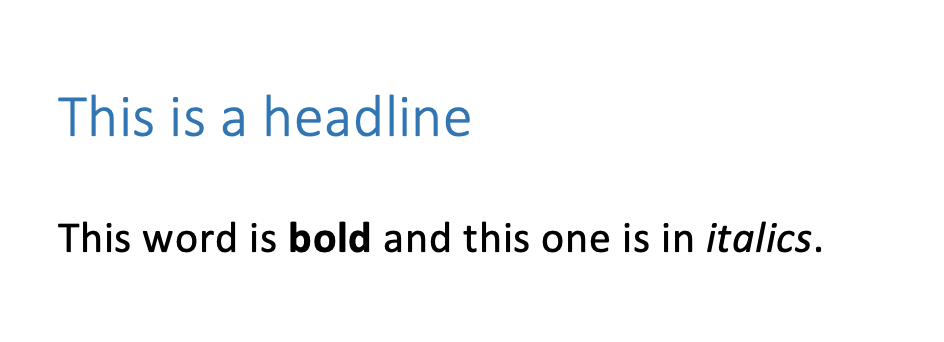
\includegraphics[scale=.3]{../../texfiles-beamer/tex-material/WissArb-latex/WYSIWYG}
	\end{figure}
		
	\item \LaTeX : \textbf{WYGIWYN} or \textbf{WYGIWYM} (\emph{what-you-get-is-what-you-need}/\emph{mean})
	
	\begin{figure}
		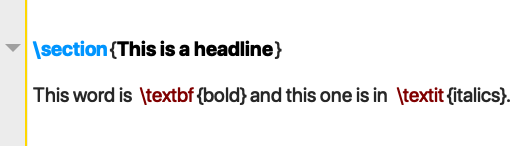
\includegraphics[scale=.3]{../../texfiles-beamer/tex-material/WissArb-latex/WYSIWYM}
	\end{figure}
	
\end{itemize}\end{frame}


%%%%%%%%%%%%%%%%%%%%%%%%%%%%%%%%%%%
%%%%%%%%%%%%%%%%%%%%%%%%%%%%%%%%%%%
%\subsection{Warum sollte ich es benutzen?}
%%\frame{
%%	%\frametitle{~}
%%	\begin{multicols}{2}
%%		\tableofcontents[currentsection,hideallsubsections]
%%	\end{multicols}
%%}
%%
%%%%%%%%%%%%%%%%%%%%%%%%%%%%%%%%%%%
%
%\begin{frame}
%\frametitle{Warum sollte ich es benutzen?}
%
%\begin{itemize}
%	\item Zeitersparnis ({\tiny nicht am Anfang!})
%	\item[]
%
%\pause	
%
%	\item Man hört auf, Sachen zu tun, die der Computer für einen erledigen kann. Daher hat man mehr Zeit, um sich mit dem Inhalt zu befassen.
%	\item[]
%
%\pause	
%
%	\item Die Texte werden sehr gut gesetzt!
%	\item[]
%
%\pause
%
%	\item Ein Programm für alle Funktionen: Artikel, Bücher, Poster, Präsentationen, \dots 
%	\item[]
%
%\pause
%
%	\item Gratis!!
%
%\end{itemize}
%
%\end{frame}


%%%%%%%%%%%%%%%%%%%%%%%%%%%%%%%%%%%
%%%%%%%%%%%%%%%%%%%%%%%%%%%%%%%%%%%
\iftoggle{handout}{
	
%%%%%%%%%%%%%%%%%%%%%%%%%%%%%%%%%%%

%%%%%%%%%%%%%%%%%%%%%%%%%%%%%%%%%%
%%%%%%%%%%%%%%%%%%%%%%%%%%%%%%%%%%
\subsection{Examples}
%\frame{
%	%\frametitle{~}
%	\begin{multicols}{2}
%		\tableofcontents[currentsection,hideallsubsections]
%	\end{multicols}
%}
%%%%%%%%%%%%%%%%%%%%%%%%%%%%%%%%%%%

\begin{frame}
\frametitle{Examples}

What can you do with \LaTeX ?

\end{frame}


%%%%%%%%%%%%%%%%%%%%%%%%%%%%%%%%%%%%
\begin{frame}
\frametitle{Books \& Articles}

%\begin{figure}[htbp]

\begin{minipage}[c]{0.49\textwidth}
\centering
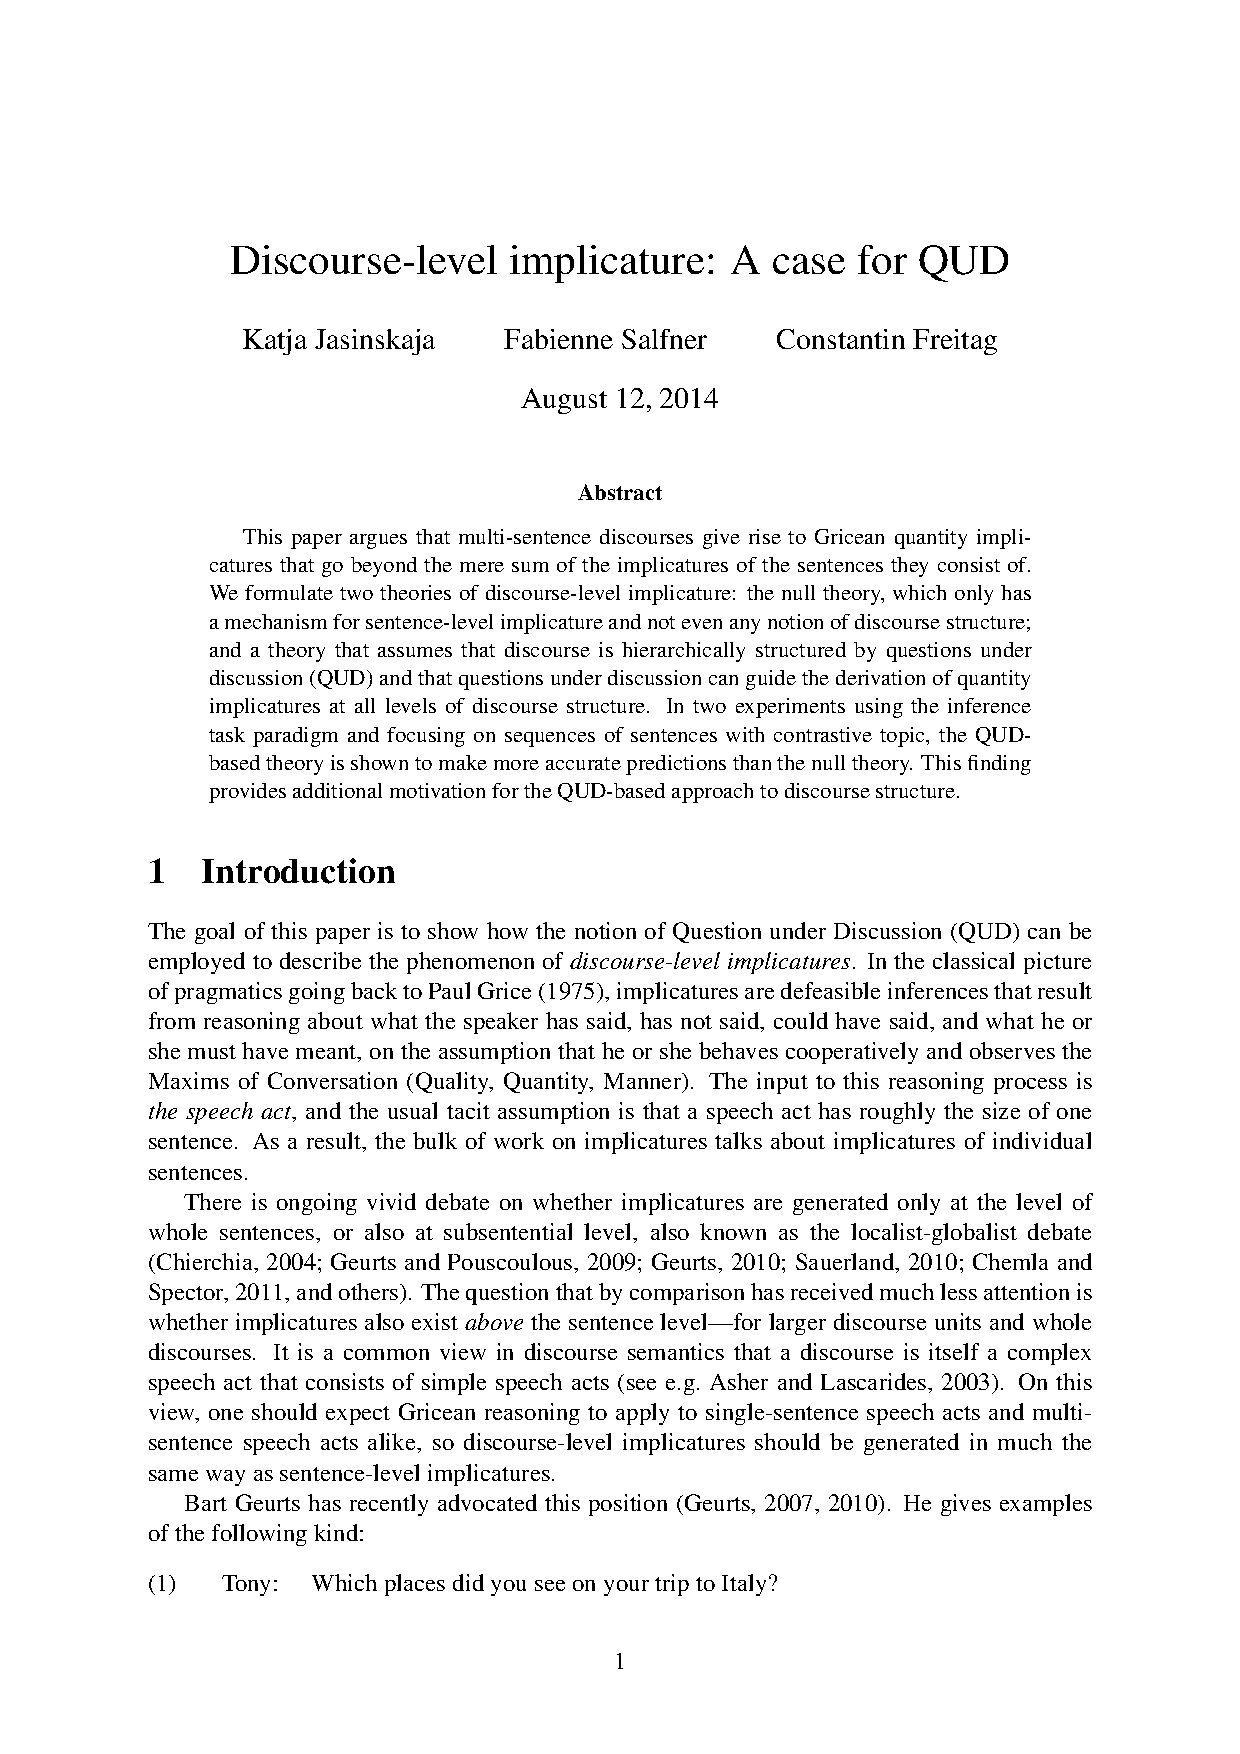
\includegraphics[width=0.80\linewidth]{../../texfiles-beamer/tex-material/WissArb-latex/LaTeX_article.pdf}
\end{minipage}  
%  
\begin{minipage}[c]{0.49\textwidth}
\centering
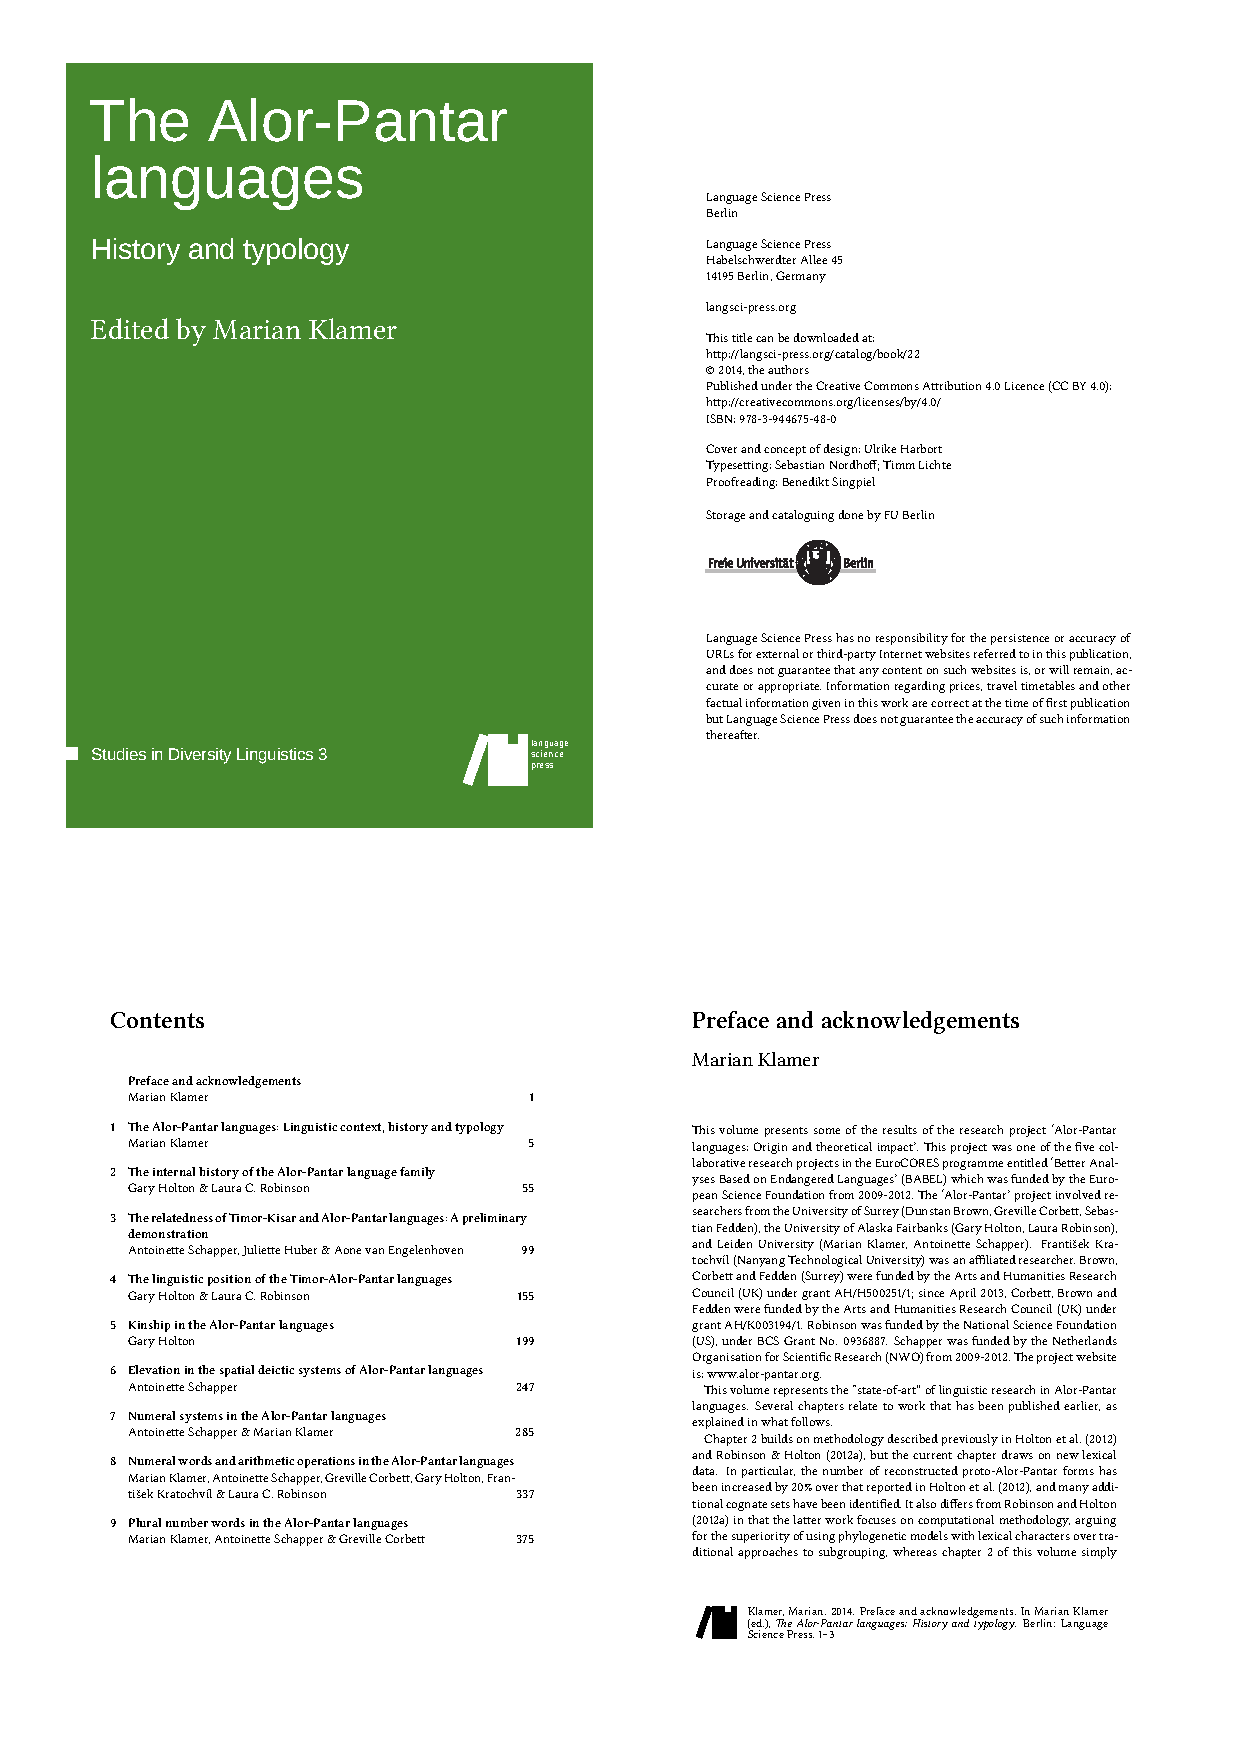
\includegraphics[width=0.80\linewidth]{../../texfiles-beamer/tex-material/WissArb-latex/LaTeX_book_2.pdf}
%\caption{Adjunkt und Komplement}	
\end{minipage}
%         
%\end{figure}

\end{frame}


%%%%%%%%%%%%%%%%%%%%%%%%%%%%%%%%%%%%
\begin{frame}
\frametitle{Poster \& Letter}

%\begin{figure}[b]

\begin{minipage}[b]{0.49\textwidth}
\centering
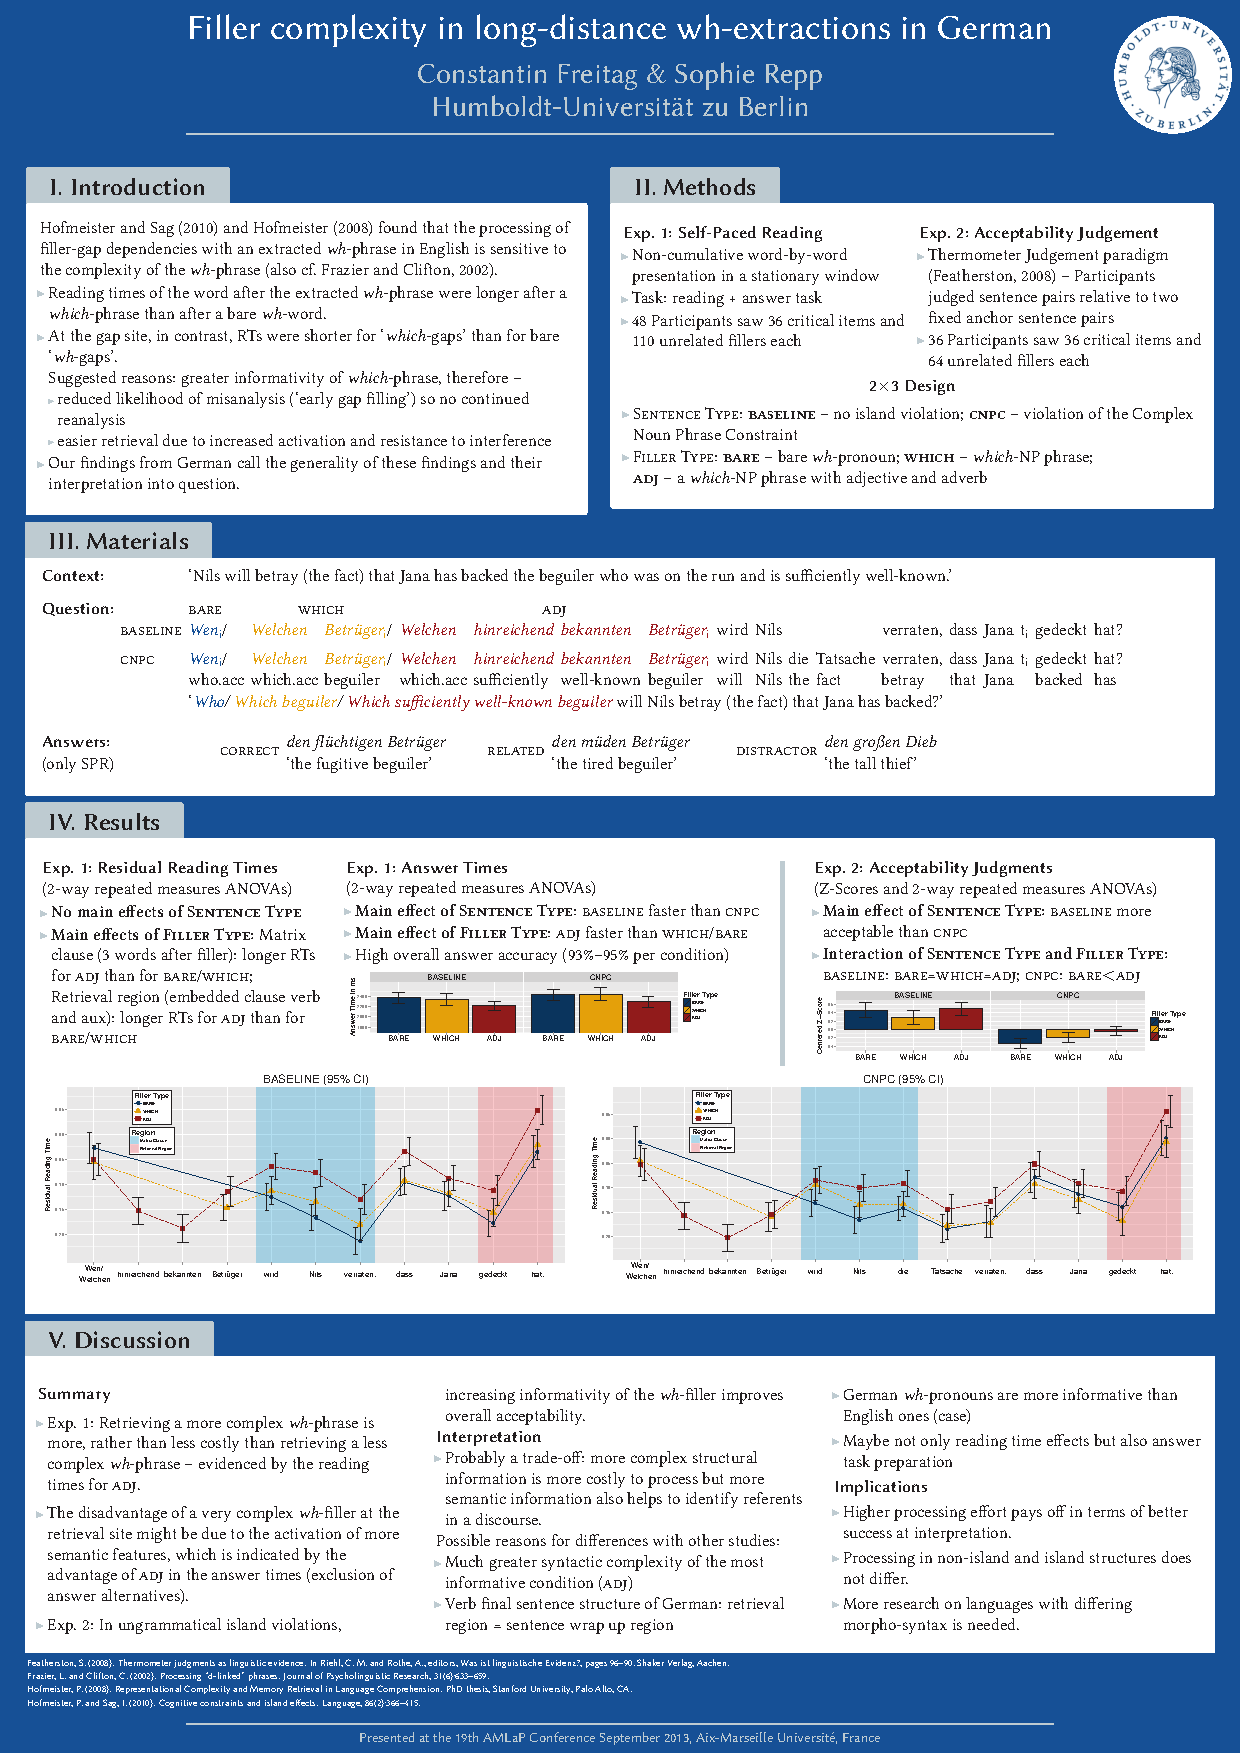
\includegraphics[width=0.80\linewidth]{../../texfiles-beamer/tex-material/WissArb-latex/Freitag_Repp_AMLaP_2013_A4.pdf}
\end{minipage}  
%  
\begin{minipage}[b]{0.49\textwidth}
\centering

\includegraphics[width=0.80\linewidth]{../../texfiles-beamer/tex-material/WissArb-latex/UKN_brief.pdf}
%\caption{Adjunkt und Komplement}	
\end{minipage}
%         
%\end{figure}

\end{frame}


%%%%%%%%%%%%%%%%%%%%%%%%%%%%%%%%%%%
\begin{frame}
\frametitle{Trees}

\begin{figure}

\begin{minipage}[b]{0.70\textwidth}
\centering
\footnotesize{
\begin{forest}
%sn edges,
[IP 
	[DP [Peter\\
	\emph{Peter},roof]]
	[\xprime{I} 
		[VP 
			[\xprime{V} 
				[DP [den Wagen\\
				\emph{the car}, roof]]
				[\xzero{V} [t$_{i}$,draw]{
				\draw[->,dotted] () to[out=south east,in=south] (IHead);}
				]
			]
		]
		[\xzero{I} 
			[\alert{kauft}$_{i}$\\
			\emph{buys},name=IHead]
		]{\draw[<-,red] (.south east)--++(0em,-1.5ex)--++(+2em,0pt)
node[anchor=west,align=center]{finite};}
	]
]
\end{forest}
}
\caption{Head movement}	
\end{minipage} 

\end{figure}

\end{frame}


%%%%%%%%%%%%%%%%%%%%%%%%%%%%%%%%%%%
\begin{frame}
\frametitle{Glossing \& IPA}

\ea 
	\ea
	\gll Der Mann schläf -t.\\
	the.\textsc{nom} man.\textsc{nom} sleep -s\\
	\glt `The man is sleeping.'

	\ex 
	%\settowidth\jamwidth{\textsc{Deutsch}}
	\gll Der Mann hat dem Jungen ein Buch über Linguistik gegeben.\\
	the.\textsc{nom} man.\textsc{nom} has the.\textsc{dat} boy.\textsc{dat} a.\textsc{acc} book.\textsc{acc} about linguistics give.\textsc{ptcp.prf}\\
	\glt `The man gave the boy a book about linguistics.' 
	%\jambox{\textsc{Deutsch}}
	\z 
		
\ex 
	\ea \ab{phonetics} 
	\ex {/}\textipa{f@".nE.tIks}/ 
	\ex {[}\textipa{f@"nEtIks}] 
	\z 
\z 

\end{frame}

}
%% END handout true 
%% BEGIN handout false
{
%%%%%%%%%%%%%%%%%%%%%%%%%%%%%%%%%%

%% EMPTY

}%% END HO-Toggle
%%%%%%%%%%%%%%%%%%%%%%%%%%%%%%%%%%


%%%%%%%%%%%%%%%%%%%%%%%%%%%%%%%%%%%
%%%%%%%%%%%%%%%%%%%%%%%%%%%%%%%%%%%
\subsection{How does \LaTeX\ work?}
%\frame{
%	%\frametitle{~}
%	\begin{multicols}{2}
%		\tableofcontents[currentsection,hideallsubsections]
%	\end{multicols}
%}
%%%%%%%%%%%%%%%%%%%%%%%%%%%%%%%%%%%

\begin{frame}
\frametitle{How does \LaTeX\ work?}

By compiling your document, \LaTeX\ creates further \textbf{auxiliary files} to improve the next compilations.

\begin{columns}

\column[t]{.6\textwidth}

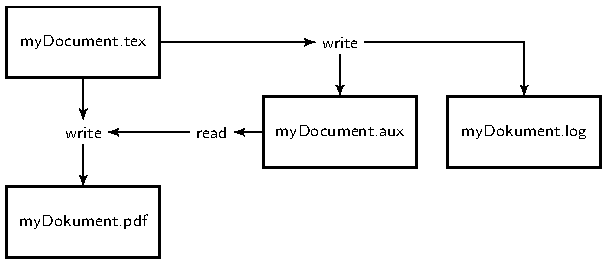
\includegraphics[scale=.75]{../../texfiles-beamer/tex-material/WissArb-latex/LaTeX-flowchart-1.pdf}

\column[t]{.4\textwidth}

\begin{itemize}
	\item your document: \ltxterm{.tex}
	\item your product: \ltxterm{.pdf}
\end{itemize}

\end{columns}

\end{frame}


%%%%%%%%%%%%%%%%%%%%%%%%%%%%%%%%%%%
\begin{frame}
%\frametitle{Wie funktioniert \LaTeX ?}

\begin{minipage}{.58\textwidth}

The auxiliary files can be \textbf{deleted} after your work is done. They will be created again when you compile.

\begin{itemize}
	\item \ltxterm{.log} \ras information about the compiling process
	
	\item \ltxterm{.bbl} \ras information for the bibliography
	
	\item \ltxterm{.nav} \ras information for the navigation through slides
	
	\item \ltxterm{.toc} \ras information for the table of contents
		
	\item \dots 
\end{itemize}

\end{minipage}
%
\begin{minipage}{.40\textwidth}
	\centering
	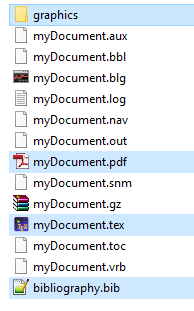
\includegraphics[width=.9\linewidth]{../../texfiles-beamer/tex-material/WissArb-latex/latexDateien}
	
\end{minipage}

\end{frame}


%%%%%%%%%%%%%%%%%%%%%%%%%%%%%%%%%%%
\begin{frame}
%\frametitle{Wie funktioniert \LaTeX ?}

\begin{minipage}{.58\textwidth}
	The following files are important and \textbf{should not be deleted}. They are not created in the compiling process:
		
	\begin{itemize}
		\item \texttt{.tex} \ras this is the document you are working on.
		
		\item \texttt{.pdf} \ras you can delete your PDF, but this is what you normally want as your result
		
		\item \texttt{.bib} \ras this file contains your bibliography data base (if you have one)
		
		\item folder \texttt{graphics} \ras here could be your graphics (if you need some)
	\end{itemize}
	
\end{minipage}
%
\begin{minipage}{.40\textwidth}
	\centering
	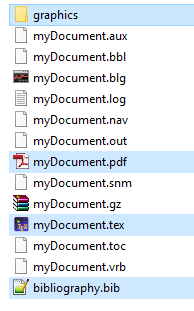
\includegraphics[width=.9\linewidth]{../../texfiles-beamer/tex-material/WissArb-latex/latexDateien}
	
\end{minipage}

\end{frame}


%%%%%%%%%%%%%%%%%%%%%%%%%%%%%%%%%%%%
%%%%%%%%%%%%%%%%%%%%%%%%%%%%%%%%%%%%
%\subsection{Software}
%%\frame{
%%	%\frametitle{~}
%%	\begin{multicols}{2}
%%		\tableofcontents[currentsection,hideallsubsections]
%%	\end{multicols}
%%}
%%%%%%%%%%%%%%%%%%%%%%%%%%%%%%%%%%%%
%
%\begin{frame}
%\frametitle{Software}
%
%In diesem Kurs werden wir mit dem \textbf{Editor} \texttt{TeXstudio} arbeiten, welcher folgende Vorteile anbietet: 
%
%\begin{itemize}
%	\item kostenlos, 
%	
%	\item kompatible mit Linux-, Windows- und Mac OS-Rechnern,
%	\item Unicode-Unterstützung, Rechtschreibkontrolle, Autovervollständigung von Befehlen, PDF-Viewer,
%	\item einfach zu verwenden und zu konfigurieren, \dots
%\end{itemize}
%
%Außer dem Editor benötigt man eine \LaTeX -\textbf{Distribution}.
%In diesem Fall werden wir \texttt{MiKTeX} (für Windows-User)
%verwenden. Für Linux-User ist \texttt{TeXLive} eine sehr bekannte Alternative und für Mac OS-User \texttt{MacTeX}. \textbf{Zuerst} soll die Distribution (\zB \texttt{MiKTeX}) und erst dann der Editor (\zB \texttt{TeXstudio}) installiert werden!
%
%\end{frame}


%%%%%%%%%%%%%%%%%%%%%%%%%%%%%%%%%%%
%%%%%%%%%%%%%%%%%%%%%%%%%%%%%%%%%%%
\section{Document structure 1}
\frame{
	%\frametitle{~}
	\begin{multicols}{2}
		\tableofcontents[currentsection,hideallsubsections]
	\end{multicols}
}
%%%%%%%%%%%%%%%%%%%%%%%%%%%%%%%%%%%

\begin{frame}[fragile]
\frametitle{Document structure 1}

A \LaTeX document consists of (at least) two parts: \textbf{preamble} and \textbf{body}.

\begin{block}{\LaTeX\ preamble}
	part of the document where \textbf{global characteristics} of the document are specified.
\end{block}

	\begin{itemize}
		\item The preamble \textbf{begins} (\textbf{obligatorily}) with the \lstinline|\documentclass{}| command.
		
		\item In the preamble you will install \textbf{packages} for further \LaTeX\ functions.
		
		\item \textbf{Optional} (either in the preamble or in the body -- preferably in the preamble)

		\begin{itemize}
			\item your \textbf{own commands} and 
			
			\item \textbf{metadata} 
		\end{itemize}
		
		\item The preamble \textbf{ends} with the command  \lstinline|\begin{document}|.
		
	\end{itemize}

\end{frame}


%%%%%%%%%%%%%%%%%%%%%%%%%%%%%%%%%
\begin{frame}[fragile]
%\frametitle{Dokumentstruktur}


\begin{block}{\LaTeX\ body}
	part of the document where \textbf{local characteristics} of the document are specified and where you write your document.
\end{block}


\begin{itemize}
	
	\item The body \textbf{begins} with the \lstinline|\begin{document}| command  (end of preambel).
	
	\item The body \textbf{ends} with \lstinline|\end{document}|. 
	
	\item[]
	
	\item Everything following the command \lstinline|\end{document}| will not be interpreted by \LaTeX .
\end{itemize}

\end{frame}


%%%%%%%%%%%%%%%%%%%%%%%%%%%%%%%%%
\begin{frame}[fragile]
\frametitle{Exercise}

Insert the following lines in your \ltxterm{.tex} file and compile.

\vspace{.5cm}

%\begin{figure}[b]

\centering
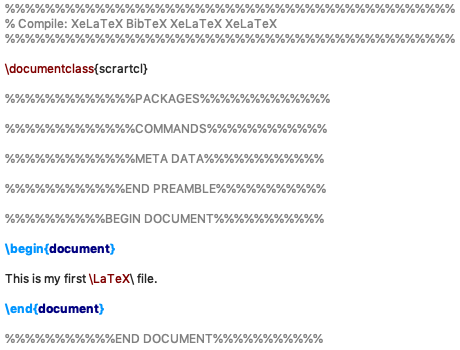
\includegraphics[scale=0.45]{../../texfiles-beamer/tex-material/WissArb-latex/xelatexTest1tex}

%	\caption{Präambel 1}
%\end{figure}
%
%
%\begin{figure}[b]

\centering

\includegraphics[width=0.86\linewidth]{../../texfiles-beamer/tex-material/WissArb-latex/latexTest1pdf}

%	\caption{Präambel 2}
%\end{figure}


\end{frame}


%%%%%%%%%%%%%%%%%%%%%%%%%%%%%%%%%
\begin{frame}[fragile]
%\frametitle{Dokumentstruktur}

\centering
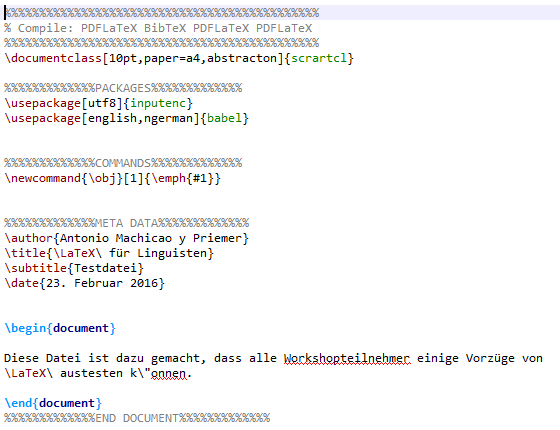
\includegraphics[width=0.9\linewidth]{../../texfiles-beamer/tex-material/WissArb-latex/latexTest2tex}


\end{frame}


%%%%%%%%%%%%%%%%%%%%%%%%%%%%%%%%%
\begin{frame}[fragile]
%\frametitle{Dokumentstruktur}

\centering

\includegraphics[width=0.99\linewidth]{../../texfiles-beamer/tex-material/WissArb-latex/latexTest2pdf}

\end{frame}


%%%%%%%%%%%%%%%%%%%%%%%%%%%%%%%%%%%%
%%%%%%%%%%%%%%%%%%%%%%%%%%%%%%%%%%%%
\subsection{Dokumentklasse}
%\frame{
%	%\frametitle{~}
%	\begin{multicols}{2}
%		\tableofcontents[currentsection,hideallsubsections]
%	\end{multicols}
%}
%%%%%%%%%%%%%%%%%%%%%%%%%%%%%%%%%%%

\begin{frame}[fragile]
\frametitle{Dokumentklasse}

Der \lstinline|documentclass|-Befehl legt die \textbf{Parameter des allgemeinen Dokument-Layouts} fest. Die wichtigsten Klassen sind: 

\begin{itemize}
\item \texttt{book} für Bücher  
\item \texttt{report} für längere Schriften mit etlichen Kapiteln, z.\,B. eine Dissertation
\item \texttt{article} für Artikel, ohne Kapitel nur mit Abschnitten
\item \texttt{letter} für Briefe
\end{itemize}


\end{frame}


%%%%%%%%%%%%%%%%%%%%%%%%%%%%%%%%%%%%
\begin{frame}[fragile]

Da diese Klassen häufig für \textbf{amerikanische Formate}
spezifiziert sind, gibt es Varianten dieser Klassen, die von
\textbf{\texttt{KOMA-Script}} zur Verfügung gestellt werden (die wir verwenden werden):

\begin{itemize}
\item \texttt{scrbook} für Bücher  
\item \texttt{scrreprt} für längere Schriften mit etlichen Kapiteln, z.\,B. eine Dissertation
\item \texttt{scrartcl} für Artikel, ohne Kapitel nur mit Abschnitten
\item \texttt{scrlttr2} für Briefe
\end{itemize}

Für Details über das \texttt{KOMA-Script} siehe \citet{Kohm&Co13a} und \url{https://www.komascript.de/}
\end{frame}


%%%%%%%%%%%%%%%%%%%%%%%%%%%%%%%%%
\begin{frame}[fragile]
%\frametitle{Dokumentstruktur}

\centering
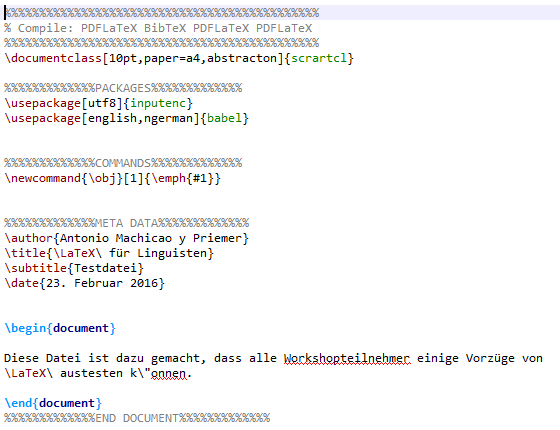
\includegraphics[width=0.9\linewidth]{../../texfiles-beamer/tex-material/WissArb-latex/latexTest2tex}


\end{frame}

%%%%%%%%%%%%%%%%%%%%%%%%%%%%%%%%%%%
\begin{frame}[fragile]
%\frametitle{Dokumentklasse}

Zudem kann man die Optionen dieser Dokumentklassen in dem \ltxterm{documentclass}-Befehl festlegen.

Häufigste Optionen und Minimalbeispiel:

\begin{itemize}
\item \textbf{Schriftgröße} für die (Default-)Schriftgröße: \ltxterm{10pt}, \texttt{11pt}, \texttt{12pt} \par
Default $\rightarrow$ \ltxterm{10pt} 

\item \textbf{Papierformat}: \ltxterm{letterpaper}, \ltxterm{a4paper} \par
Default $\rightarrow$ \ltxterm{letterpaper} \par
\end{itemize}


In den \ltxterm{KOMA-Script}-Klassen sollte man \ltxterm{paper=a4}
oder \ltxterm{paper=letter} statt \ltxterm{a4paper} bzw. \ltxterm{letterpaper} verwenden.

\end{frame}


%%%%%%%%%%%%%%%%%%%%%%%%%%%%%%%%%%%
\begin{frame}[fragile]
\frametitle{Dokumentklasse}

\begin{lstlisting}
\documentclass[10pt,paper=a4]{scrartcl}
\begin{document}
Text Text Text
\end{document}
\end{lstlisting}

\begin{description}
\item[Hinweis:] \ltxterm{TeXstudio} bietet einen Assistenten, der die Präambel für Sie schreibt. Schauen Sie in der Toolbar unter \texttt{Assistenten/Assistent für ein neues Dokument} nach. Dort können Sie alles weitere einstellen.
\end{description}

\end{frame}


%%%%%%%%%%%%%%%%%%%%%%%%%%%%%%%%%%%
%%%%%%%%%%%%%%%%%%%%%%%%%%%%%%%%%%%
\section{Befehle}
\frame{
	%\frametitle{~}
	\begin{multicols}{2}
		\tableofcontents[currentsection,hideallsubsections]
	\end{multicols}
}
%%%%%%%%%%%%%%%%%%%%%%%%%%%%%%%%%%%

\begin{frame}[fragile]
\frametitle{Befehle (commands)}


\begin{itemize}
	\item \LaTeX\ arbeitet mit einer \textbf{logischen Textauszeichnung}
	
	\item[]
	
	\item Wenn Sie etwas kursiv setzen wollen, müssen Sie nicht irgendwo \gqq{klicken}, sondern \textbf{einen Befehl eingeben}
\end{itemize}

\end{frame}


%%%%%%%%%%%%%%%%%%%%%%%%%%%%%%%%%%%
\begin{frame}[fragile]
%\frametitle{Befehle}

\textbf{Syntax von Befehlen:}

\pause

\begin{itemize}
	\item Alle \LaTeX -Befehle beginnen mit einem \textbf{Backslash} \gqq{\textbackslash}, 
	
	\item gefolgt vom \textbf{Namen des Befehls}, 
	
	\item von optionalen Argumenten in \textbf{eckigen Klammern} und 
	
	\item von obligatorischen Argumenten in \textbf{geschweiften Klammern}.

%\pause 
		
\begin{lstlisting}
\Befehlsname[optional]{obligatorisch} 
\Befehlsname[opt1, opt2=Wert]{obl1}{obl2}
\end{lstlisting}

\pause 
	
	\item Beispiele:
		
\begin{lstlisting}
\textbf{fettgedruckter Text} 
\citep[vgl.][3--5]{Freitag&MyP15a}
\end{lstlisting}

\pause 
	
	\ea \textbf{fettgedruckter Text} 
	\ex \citep[vgl.][3--5]{Freitag&MyP15a}
	\z 
\end{itemize}

\end{frame}


%%%%%%%%%%%%%%%%%%%%%%%%%%%%%%%%%%%

\begin{frame}[fragile]
%\frametitle{Befehle}

\LaTeX\ kennt im Prinzip \textbf{drei Arten von Befehlen}:

\begin{itemize}

\item[]
\item \textbf{Einfache Befehle:}

Backslash \gqq{\textbackslash} + Befehlsnamen + optionale Argumenten in eckigen Klammern + obligatorische Argumenten in geschweiften Klammern


\begin{lstlisting}
\Befehlsname[optional]{obligatorisch} 
\Befehlsname[opt1, opt2=Wert]{obl1}{obl2}
\end{lstlisting}

\pause 

\item[]
\item Beispiele:

\begin{lstlisting}
\textit{kursive Hervorhebung} 
\citet[vgl.][3--5]{Freitag&MyP15a}
\end{lstlisting}

\pause 

\ea \textit{kursive Hervorhebung} 
\ex \citet[vgl.][3--5]{Freitag&MyP15a}
\z 

\end{itemize}

\end{frame}


%%%%%%%%%%%%%%%%%%%%%%%%%%%%%%%%%%%

\begin{frame}[fragile]
%\frametitle{Befehle}


\begin{itemize}
	\item \textbf{Umgebungen:}\\
	Umgebungen bestehen aus einem \texttt{begin}- und einem \texttt{end}-Befehl. Der Befehl gilt im Bereich zwischen \texttt{begin} und \texttt{end}.

\begin{lstlisting}
\begin{Umgebung}[optional]
...
\end{Umgebung}
\end{lstlisting}

	\pause 
	
%	\item[]
	\item Beispiele:
	
\begin{lstlisting}
\begin{multicols}{2}[Beispiel]
Das ist die erste Spalte

Das ist die zweite Spalte
\end{multicols}
\end{lstlisting}
	
	\pause 
			
\ea 
\begin{multicols}{2}[Beispiel]
	Das ist die erste Spalte
		
	Das ist die zweite Spalte
\end{multicols}

\z 

\end{itemize}

\end{frame}


%%%%%%%%%%%%%%%%%%%%%%%%%%%%%%%%%
\begin{frame}[fragile,fragile]
%\frametitle{Befehle}

\begin{itemize}
\item \textbf{Deklarationen:}

Deklarationen verändern Parameter. 

Der \textbf{Skopus} von Deklarationen kann so definiert sein, dass er an bestimmten Grenzen -- wie an einem Absatzschluss -- endet, oder dass er nur auf einen \textbf{von geschweiften Klammern bestimmten Skopus} beschränkt ist.

\begin{lstlisting}
\Deklaration ... [Skopusende]
{\Deklaration ...} ausserhalb des Skopus
\end{lstlisting}

	\pause 

%	\item[]
\item Beispiele:

\begin{lstlisting}
{\small Hello world!} \Huge Hello world!
\end{lstlisting}

\pause 

\ea 
{\tiny Hello world!} \Huge Hello world!

\z 

\end{itemize}

\end{frame}


%%%%%%%%%%%%%%%%%%%%%%%%%%%%%%%%%%%
%%%%%%%%%%%%%%%%%%%%%%%%%%%%%%%%%%%
\section{Zeichen \& Umbrüche}
\frame{
	%\frametitle{~}
	\begin{multicols}{2}
		\tableofcontents[currentsection,hideallsubsections]
	\end{multicols}
}
%%%%%%%%%%%%%%%%%%%%%%%%%%%%%%%%%%%


%%%%%%%%%%%%%%%%%%%%%%%%%%%%%%%%%%%
%%%%%%%%%%%%%%%%%%%%%%%%%%%%%%%%%%%
\subsection{Zeichen \& Sonderzeichen}
%\frame{
%	%\frametitle{~}
%	\begin{multicols}{2}
%		\tableofcontents[currentsection,hideallsubsections]
%	\end{multicols}
%}
%%%%%%%%%%%%%%%%%%%%%%%%%%%%%%%%%%%

\begin{frame}[fragile]
\frametitle{Zeichen \& Sonderzeichen}

\begin{itemize}
\item Die folgenden Zeichen können problemlos verwendet werden:\\ 

\begin{lstlisting}
a...z  A...Z  0...9
. , : ; ? ! ` ' " ( ) [ ] + - * =
\end{lstlisting}

\item[]

\item Achten Sie darauf, welche Art von \textbf{Anführungszeichen} durch \lstinline|` ' "|  generiert werden \citep[vgl.][]{MyP17c}. 

\item[]

\item Die \textbf{Umlaute} \gqq{ä, ö, Ä, Ö, \dots}, \textbf{Akzente} \gqq{á, à, \dots} und das \textbf{Eszett} \gqq{ß} können (bei PDF-\LaTeX ) mithilfe des folgenden Pakets \lstinline|\usepackage[utf8]{inputenc}| direkt eingegeben werden.

Andernfalls müssen sie mit Extrabefehlen geschrieben werden:


\begin{lstlisting}
\"A \"O \"a \"o \'a \`o \ss{} 
oder \"{A} {\"O} {\ss} 
\end{lstlisting}

\ea \"A \"O \"a \"o \'a \`o \ss{} oder \"{A} {\"O} {\ss} 
\z 

\end{itemize}

\end{frame}


%%%%%%%%%%%%%%%%%%%%%%%%%%%%%%%%%%%
\begin{frame}[fragile]
%\frametitle{Zeichen und Sonderzeichen}

\begin{itemize}
	
	\item Die folgenden Zeichen haben in \LaTeX\ eine \textbf{besondere Bedeutung} und können nicht einfach im Fließtext verwendet werden:
	
\begin{lstlisting}
#  $  &  ~  _  ^  {  }  <  >  |  \  %
\end{lstlisting}

	\item[]

\pause

	\item Um diese Zeichen verwenden zu können, musst man den in \LaTeX\ vordefinierten Funktionen dieser Zeichen \textbf{entkommen}. Bei einigen Zeichen kann man den vordefinierten Funktionen durch \textbf{Voranstellen eines Backslashs} entkommen. 

\begin{lstlisting}
\#  \$  \&  \_  \{  \}  \%
\end{lstlisting}
	
\end{itemize}

\end{frame}


%%%%%%%%%%%%%%%%%%%%%%%%%%%%%%%%%%%
\begin{frame}[fragile]
%\frametitle{(Sonder-)Zeichen}

\begin{itemize}

	\item Dem \textbf{Backslash}, der \textbf{Größer-als}- und \textbf{Kleiner-als}-Zeichen, der \textbf{Tilde}, dem \textbf{Zirkumflex} und dem \textbf{senkrechten Strich} (\emph{pipe}) kann man nicht mit dem Backslash entkommen.

\end{itemize}

\end{frame}


%%%%%%%%%%%%%%%%%%%%%%%%%%%%%%%%%%%
\begin{frame}[fragile]
%\frametitle{(Sonder-)Zeichen}

\begin{itemize}

\item Da die Folge \textbackslash\textbackslash\ für \textbf{Zeilenumbrüche} reserviert ist, kann man dem einfachen \textbf{Backslash} \gqq{\textbackslash} nicht mit Verwendung eines vorangestellten Backslashs entkommen. Dafür sollte der folgende Befehl benutzt werden:

\begin{lstlisting}
\textbackslash 
\end{lstlisting}

\item Die \textbf{Größer-als-} \gqq{\textgreater} und \textbf{Kleiner-als-Symbole} \gqq{\textless} können im Text durch die folgenden Befehle oder durch die Verwendung des Mathematikmodus', d.\,h. durch die \textbf{Klammerung in \$-Zeichen} erzeugt werden (mehr zum Mathematikmodus später).

\begin{lstlisting}
\textgreater $>$
\textless $<$
\end{lstlisting}

\end{itemize}

\end{frame}


%%%%%%%%%%%%%%%%%%%%%%%%%%%%%%%%%%%
\begin{frame}[fragile]
%\frametitle{(Sonder-)Zeichen}

\begin{itemize}

\item Um den \textbf{senkrechten Strich} (\gq{pipe}) darzustellen, kann man entweder den Befehl \textbf{\texttt{vert}} oder den Strich in der \textbf{Mathematikmodusklammerung} eingeben oder den Befehl \textbf{\texttt{textbar}} außerhalb des Mathematikmodus'.

\begin{lstlisting}
$\vert$  $|$  \textbar
\end{lstlisting}

\item[]

\item Die \textbf{Tilde} \gqq{\textasciitilde} hat in \LaTeX\ die Funktion eines geschützten Leerzeichens. Um dieser Funktion zu entkommen, kann man nicht den Backslash verwenden (\lstinline|\~|), denn dadurch erscheint der folgende Buchstabe mit einer Tilde. So bei der Eingabe \gqq{\texttt{\textbackslash\textasciitilde nicht}}, erscheint \gqq{\~nicht}. Will man auch dieser Funktion entkommen, muss der folgende Befehl (ähnlich wie bei dem Backslash) benutzt werden:

\begin{lstlisting}
\textasciitilde
\end{lstlisting}

\end{itemize}

\end{frame}


%%%%%%%%%%%%%%%%%%%%%%%%%%%%%%%%%%%%
\begin{frame}[fragile]
%\frametitle{(Sonder-)Zeichen}

\begin{itemize}
\item Das gleiche Problem taucht beim \textbf{Zirkumflex}  \gqq{\textasciicircum} auf, welcher als Akzent \zB im Französischen gebraucht wird. Daher erscheint bei der Eingabe \gqq{\texttt{s\textbackslash\textasciicircum ur}} der folgende Output: \gqq{s\^ur}. Aus diesem Grund benötigt man den folgenden Befehl um den Zirkumflex als Output zu haben:

\begin{lstlisting}
\textasciicircum
\end{lstlisting}

\item[]

\item Weiteres zu Sonderzeichen in \LaTeX :

\url{https://de.wikibooks.org/wiki/LaTeX/_Akzente_und_Sonderzeichen}

\end{itemize}

\end{frame}


%%%%%%%%%%%%%%%%%%%%%%%%%%%%%%%%%%
%%%%%%%%%%%%%%%%%%%%%%%%%%%%%%%%%%
\subsection{Leerzeichen \& Zeilenumbrüche}
%\frame{
%	%\frametitle{~}
%	\begin{multicols}{2}
%		\tableofcontents[currentsection,hideallsubsections]
%	\end{multicols}
%}
%%%%%%%%%%%%%%%%%%%%%%%%%%%%%%%%%%%

\begin{frame}
\frametitle{Leerzeichen \& Zeilenumbrüche}

\begin{itemize}
\item \LaTeX\ hat eine \textbf{gesonderte Behandlung von Leerzeichen}, die viele typographische Fehler automatisch korrigiert.

\item Es macht \textbf{keinen Unterschied} zwischen einem Leerzeichen (\gq{blank}) oder einem Tabulator (\gq{tab}).

\item Es zählt \textbf{keine aufeinanderfolgenden Leerzeichen}, d.\,h. mehrere konsekutive Leerzeichen werden nur als eins behandelt.

\item Ein Leerzeichen zu \textbf{Beginn einer Zeile} wird einfach ignoriert.

\item Ein \textbf{Zeilenumbruch} im Code wird als einzelnes Leerzeichen interpretiert.

\item Eine \textbf{Leer\emph{zeile}} (d.\,h. zwei Zeilenumbrüche hintereinander) legen das Ende eines Absatzes fest.

\item \textbf{Mehr Leerzeilen} (oder Zeilenumbrüche) werden als \emph{eine} einzelne Leerzeile interpretiert.

\end{itemize}

\end{frame}


%%%%%%%%%%%%%%%%%%%%%%%%%%%%%%%%%%%
\begin{frame}[fragile]
%\frametitle{Leerzeichen}

Hier ein Beispiel:

\begin{lstlisting}
Hier ist   ein      Beispieltext   mit   viel
zu vielen    Leerzeichen   .
In     Word   sind sie immer     zu   sehen.
Hier verwenden wir einen  
Zeilenumbruch.

Zwei Zeilenumbrüche ergeben einen neuen Absatz.



Mehr als zwei Umbrüche ergeben nur einen neuen Absatz.
\end{lstlisting}

\outputbox{
Hier ist   ein      Beispieltext   mit   viel
zu vielen    Leerzeichen   .
In     Word   sind sie immer     zu   sehen.
Hier verwenden wir einen  
Zeilenumbruch.

Zwei Zeilenumbrüche ergeben einen neuen Absatz.



Mehr als zwei Umbrüche ergeben nur einen neuen Absatz.
}

\end{frame}


%%%%%%%%%%%%%%%%%%%%%%%%%%%%%%%%%%%
%%%%%%%%%%%%%%%%%%%%%%%%%%%%%%%%%%%
\section{(Aus-)Kommentieren}
\frame{
	%\frametitle{~}
	\begin{multicols}{2}
		\tableofcontents[currentsection,hideallsubsections]
	\end{multicols}
}
%%%%%%%%%%%%%%%%%%%%%%%%%%%%%%%%%%%

\begin{frame}
\frametitle{(Aus-)Kommentieren}

Das \textbf{\%} ist das Zeichen um \LaTeX -Code auszukommentieren, d.\,h. \LaTeX\ wird den gesamten folgenden Text bis zum Zeilenumbruch \textbf{ignorieren}. Der Text nach dem Prozentzeichen wird weder interpretiert noch im Output wiedergegeben. Kommentare sind sehr hilfreich beim Programmieren. 

Durchs Auskommentieren kann man:

\begin{itemize}
\item \textbf{Code/Text verstecken}, ohne ihn zu löschen;

\item leichter in Zeilen oder größeren Regionen \textbf{Fehler} finden;

\item \textbf{Leerzeichen oder Leerzeilen} in langen Eingabezeilen \textbf{unterbinden};

\item \textbf{Kommentare in den Code schreiben}, ohne dass sie als Text gedruckt werden

\end{itemize}

\end{frame}


%%%%%%%%%%%%%%%%%%%%%%%%%%%%%%%%%%
\begin{frame}[fragile]
\frametitle{(Aus-)Kommentieren}

\begin{lstlisting}
Hier ist etwas Code, der angezeigt werden soll.
%hier sind wichtige Notizen

Kommentare können sogar ein Wort teilen: 
Rindfleischetikettierungs% Notiz: Fugen-s
überwachungsaufgaben% Notiz: Fugen-n
übertragungsgesetz. 
\end{lstlisting}

\outputbox{
Hier ist etwas Code, der angezeigt werden soll.
%hier sind wichtige Notizen

Kommentare können sogar ein Wort teilen: 
Rindfleischetikettierungs% Notiz: Fugen-s
überwachungsaufgaben% Notiz: Fugen-n
übertragungsgesetz. 
}

\end{frame}


%%%%%%%%%%%%%%%%%%%%%%%%%%%%%%%%%%%%
%%%%%%%%%%%%%%%%%%%%%%%%%%%%%%%%%%%%
\section{Hausaufgabe 0}
\frame{
	\begin{multicols}{2}
		%\frametitle{~}
		\tableofcontents[currentsection,hideallsubsections]
	\end{multicols}
}
%%%%%%%%%%%%%%%%%%%%%%%%%%%%%%%%%%%%

\begin{frame}{Hausaufgabe 0: \LaTeX -Vorbereitung}

\begin{itemize}
	\item Laden Sie \ltxpack{MiKTeX} und \ltxpack{TeXstudio} \gs{wie in der Anleitung in Moodle angegeben} herunter.
	\item[]
	
	\item Installieren Sie beide Programme.
	\item[]
	
	\item Folgen Sie dabei der Anleitung in Moodle.
	\item[]
	
	\item Falls Sie \textbf{Probleme bei der Installation} haben, melden Sie sich bitte bei Pia Linscheid \emph{vor} der nächsten Sitzung! Andernfalls werden Sie die kommenden Hausaufgaben nicht abgeben können.
	
	\item[]
	
	\item \textbf{Alternative:} Anstatt die Programme zu installieren, können Sie versuchen Ihre Hausaufgaben mit Overleaf zu lösen (Siehe Anleitung in Moodle).
\end{itemize}

\end{frame}


%%%%%%%%%%%%%%%%%%%%%%%%%%%%%%%%%%%%
\begin{frame}{Hausaufgabe 0: Lektüre}

\begin{itemize}
\item Lesen Sie den \textbf{LingStudi-Guide} (s.~Moodle/Allgemeines)
\end{itemize}

\end{frame}


%%%%%%%%%%%%%%%%%%%%%%%%%%%%%%%%%%%%
\begin{frame}{Hausaufgabe 0: Mitgestalten}

\begin{itemize}
\item Schreiben Sie bei Moodle im Bereich \gqq{Was will ich in diesem Kurs lernen?} \textbf{einen bis zwei Stichpunkte} auf. Erklären Sie kurz \gs{wenn nötig} was Sie damit meinen.

\end{itemize}

\end{frame}


%%%%%%%%%%%%%%%%%%%%%%%%%%%%%%%%%%%
%%%%%%%%%%%%%%%%%%%%%%%%%%%%%%%%%%%
%\section{XY}
%%\frame{
%%\begin{multicols}{2}
%%\frametitle{~}
%%	\tableofcontents[currentsection]
%%\end{multicols}
%%}
%%%%%%%%%%%%%%%%%%%%%%%%%%%%%%%%%%%
%
%\begin{frame}{XY}
%
%\begin{itemize}
%	\item XY
%\end{itemize}
%
%\end{frame}


%%%%%%%%%%%%%%%%%%%%%%%%%%%%%%%%%%%%
%%%%%%%%%%%%%%%%%%%%%%%%%%%%%%%%%%%%
%\iftoggle{handout}{
%	
%%%%%%%%%%%%%%%%%%%%%%%%%%%%%%%%%%%%%
%\begin{frame}
%%\frametitle{Bücher \& Artikel}
%	
%Test Toggle ON
%	
%\end{frame}
%
%}
%%% END handout true 
%%% BEGIN handout false
%{
%%%%%%%%%%%%%%%%%%%%%%%%%%%%%%%%%%%
%
%%% EMPTY
%
%}%% END HO-Toggle
%%%%%%%%%%%%%%%%%%%%%%%%%%%%%%%%%%%